%!TEX root = ../main.tex
\chapter{高亮度空间分离双频电子枪的优化设计}
\label{chap:GA}
近年来理论和实验研究指出,在光阴极上产生笔形束(纵横比远大于 1 的束团)可以提高注入器出口处束流的横向亮度,且束流的峰值流强可以通过在电子枪后放置一个微波聚束器得到提高。我们将这个结果应用于 S 波段光阴极注入器中,提出了将一个高次谐波腔紧贴 S 波段电子枪放置,就可形成一个空间分离的双频电子枪,目标是实现 200\,pC 电荷量下注入器出口处达到 30\,A 峰值流强以及 0.2\,mm$\cdot$mrad 以下的发射度。

\section{双频光阴极微波电子枪}
经过多年的模拟和实验探索,目前光阴极注入器出口处的束团横向亮度已经趋近于光阴极表面的最大束流亮度。想进一步提高束流亮度,可以提高阴极表面电场强度,降低光电发射时的电子剩余动能,或者将激光的尺寸从扁平状改变为细长状(笔形束)。光电发射时采用笔形束的基本原理是牺牲光电流的峰值流强,降低空间电荷效应,抑制发射度增长。因此如果采用笔形束方案,为保持光阴极注入器出口处流强足够(一般 FEL 的应用对注入器出口处的流强要求为 30\,A 左右),必须要使用聚束腔(buncher)。然而,由于笔形束的纵向尺寸较大,占有一定的微波相位,RF 发射度就会增长,进而束团的纵向分布在聚束后就会变得高度不对称,这样的束流对于 XFEL 等应用其出光品质就会降低。

为了降低 RF 发射度增长以及减小束团纵向分布不对称性,空间叠加型光阴极电子枪的概念应运而生。典型的空间叠加型光阴极电子枪结构见图 \ref{fig:overlapgun}。

\begin{figure}[htbp]
\centering
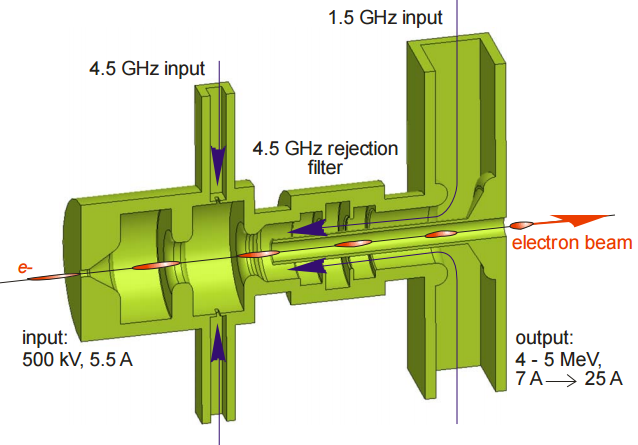
\includegraphics[width=0.6\textwidth]{overlapgun}
\caption{\label{fig:overlapgun} PSI 设计的空间叠加型光阴极电子枪结构图。}
\end{figure}

其原理为:将基模和高阶模(一般是三阶模)叠加在同一个腔体内,那么在某一段 RF 相位区间就会形成一段线性的微波场,如图 \ref{fig:linearfield} 所示。工作时将电子束置于该相位区间,则原来的微波场造成的二阶 RF 效应就被补偿,电子束从始至终处于一个线性场区,其引入的能量调制为线性,从而实现均匀的压缩,即在保持发射度以及峰值流强的情况下,使电子束的纵向分布也尽量均匀,提高后续的出光效率。

\begin{figure}[htbp]
\centering
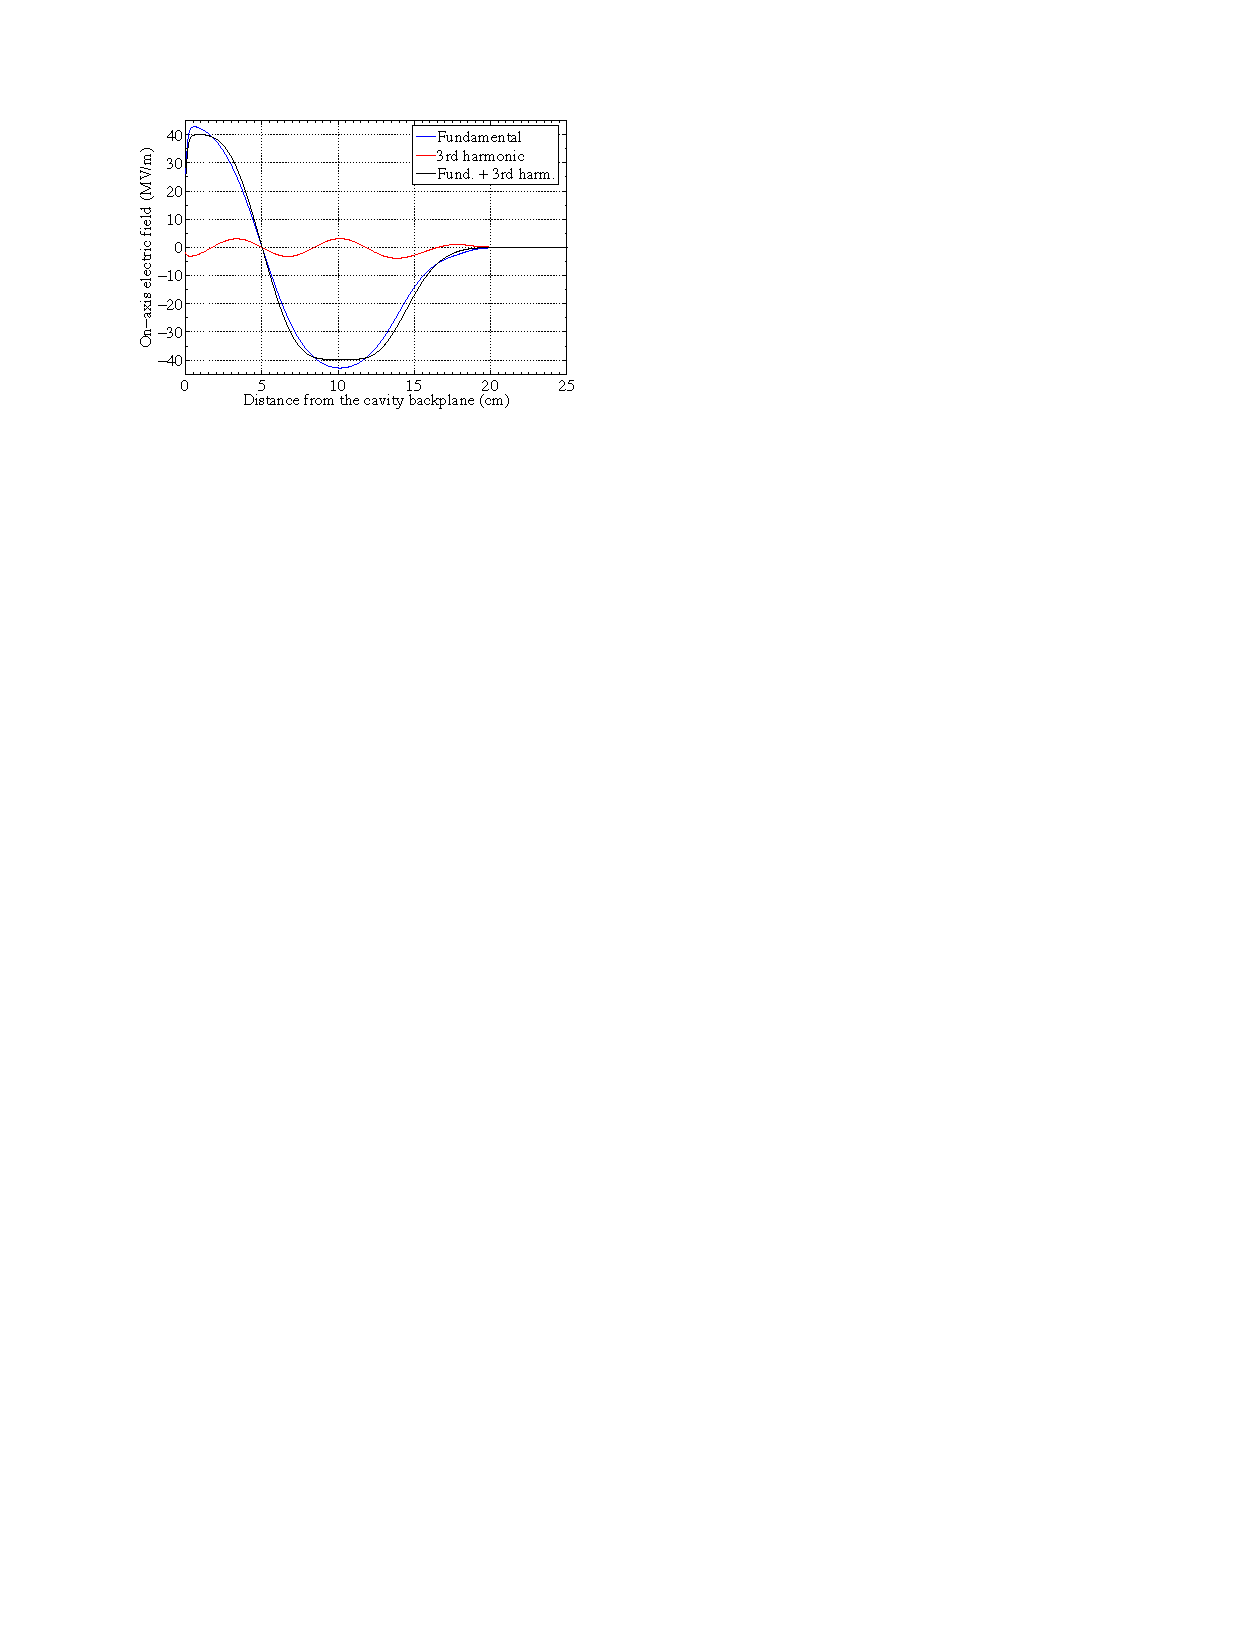
\includegraphics[width=0.6\textwidth]{overlap}
\caption{\label{fig:linearfield} 空间叠加型光阴极电子枪中的微波场。}
\end{figure}

尽管空间叠加型电子枪的原理已经由束流动力学模拟所验证,想真正实现这个想法却是很困难的:一把空间叠加型电子枪需要两个耦合器和一个过滤器,并且要在同一个腔中同时调谐和调平基模和高阶模(HOM)两个模式,其工程难度是巨大的。受此思想启发,我们提出了一种不同的路线来实现双频电子枪,即将两个 RF 模式在空间上分离开,分别将它们放在基模腔和高阶模腔中,并将基模腔和高阶模腔紧凑地组合起来,就形成了空间分离双频电子枪。

实际设计中,我们将一个 BNL 型 1.6 cell S 波段电子枪和一个高阶模腔集成在一起,初始束团的纵向尺寸先被拉长,抑制了空间电荷力发射度的增长,随后在束流经过高阶模腔时进行聚束,这样就可以在注入器出口处获得较高的峰值流强。由于相同的电荷量下,较长束团对应的横向尺寸较小,因此此举也可减小阴极表面初始热发射度。空间分离双频电子枪中的高频腔也同时可对束流纵向相空间进行线性化,从而补偿掉微波场的二阶效应,从而可在注入器出口形成对称束流,这对电子束团的后续应用有很大好处。

\section{空间分离双频电子枪的腔型设计}
我们选择了 S 波段的四阶模 X 波段作为高频腔的工作波段,并利用 Superfish 做电磁场模拟以进行腔结构参数设计。在腔型尺寸设计中,主要考察了以下几个限制条件:1)基频腔和高频腔的工作模式频率要分别为 S 波段和 X 波段;2)S 波段模式的场要调平;3)X 波段模式渗透到 S 波段腔体的场不能太强。为了同时满足三个条件,选定了 S 波段半腔半径,S 波段整腔半径与 X 波段腔半径作为输入变量;两个模式的频率,S 波段模式场平以及 X 波段模式的场渗透率(X 波段模式在 S 波段腔中最高场强与在 X 波段腔中最高场强之比)为目标变量,采用了梯度下降法进行优化。该优化方法的主要步骤如下:
\red{补充该步骤}

最终整体双频电子枪腔型及场分布见图 \ref{fig:field_sx}。S 波段腔型结构参数见表 \ref{tab:geo_s},X 波段腔型结构参数见表 \ref{tab:geo_x}。
\begin{figure}[htbp]
	\centering
	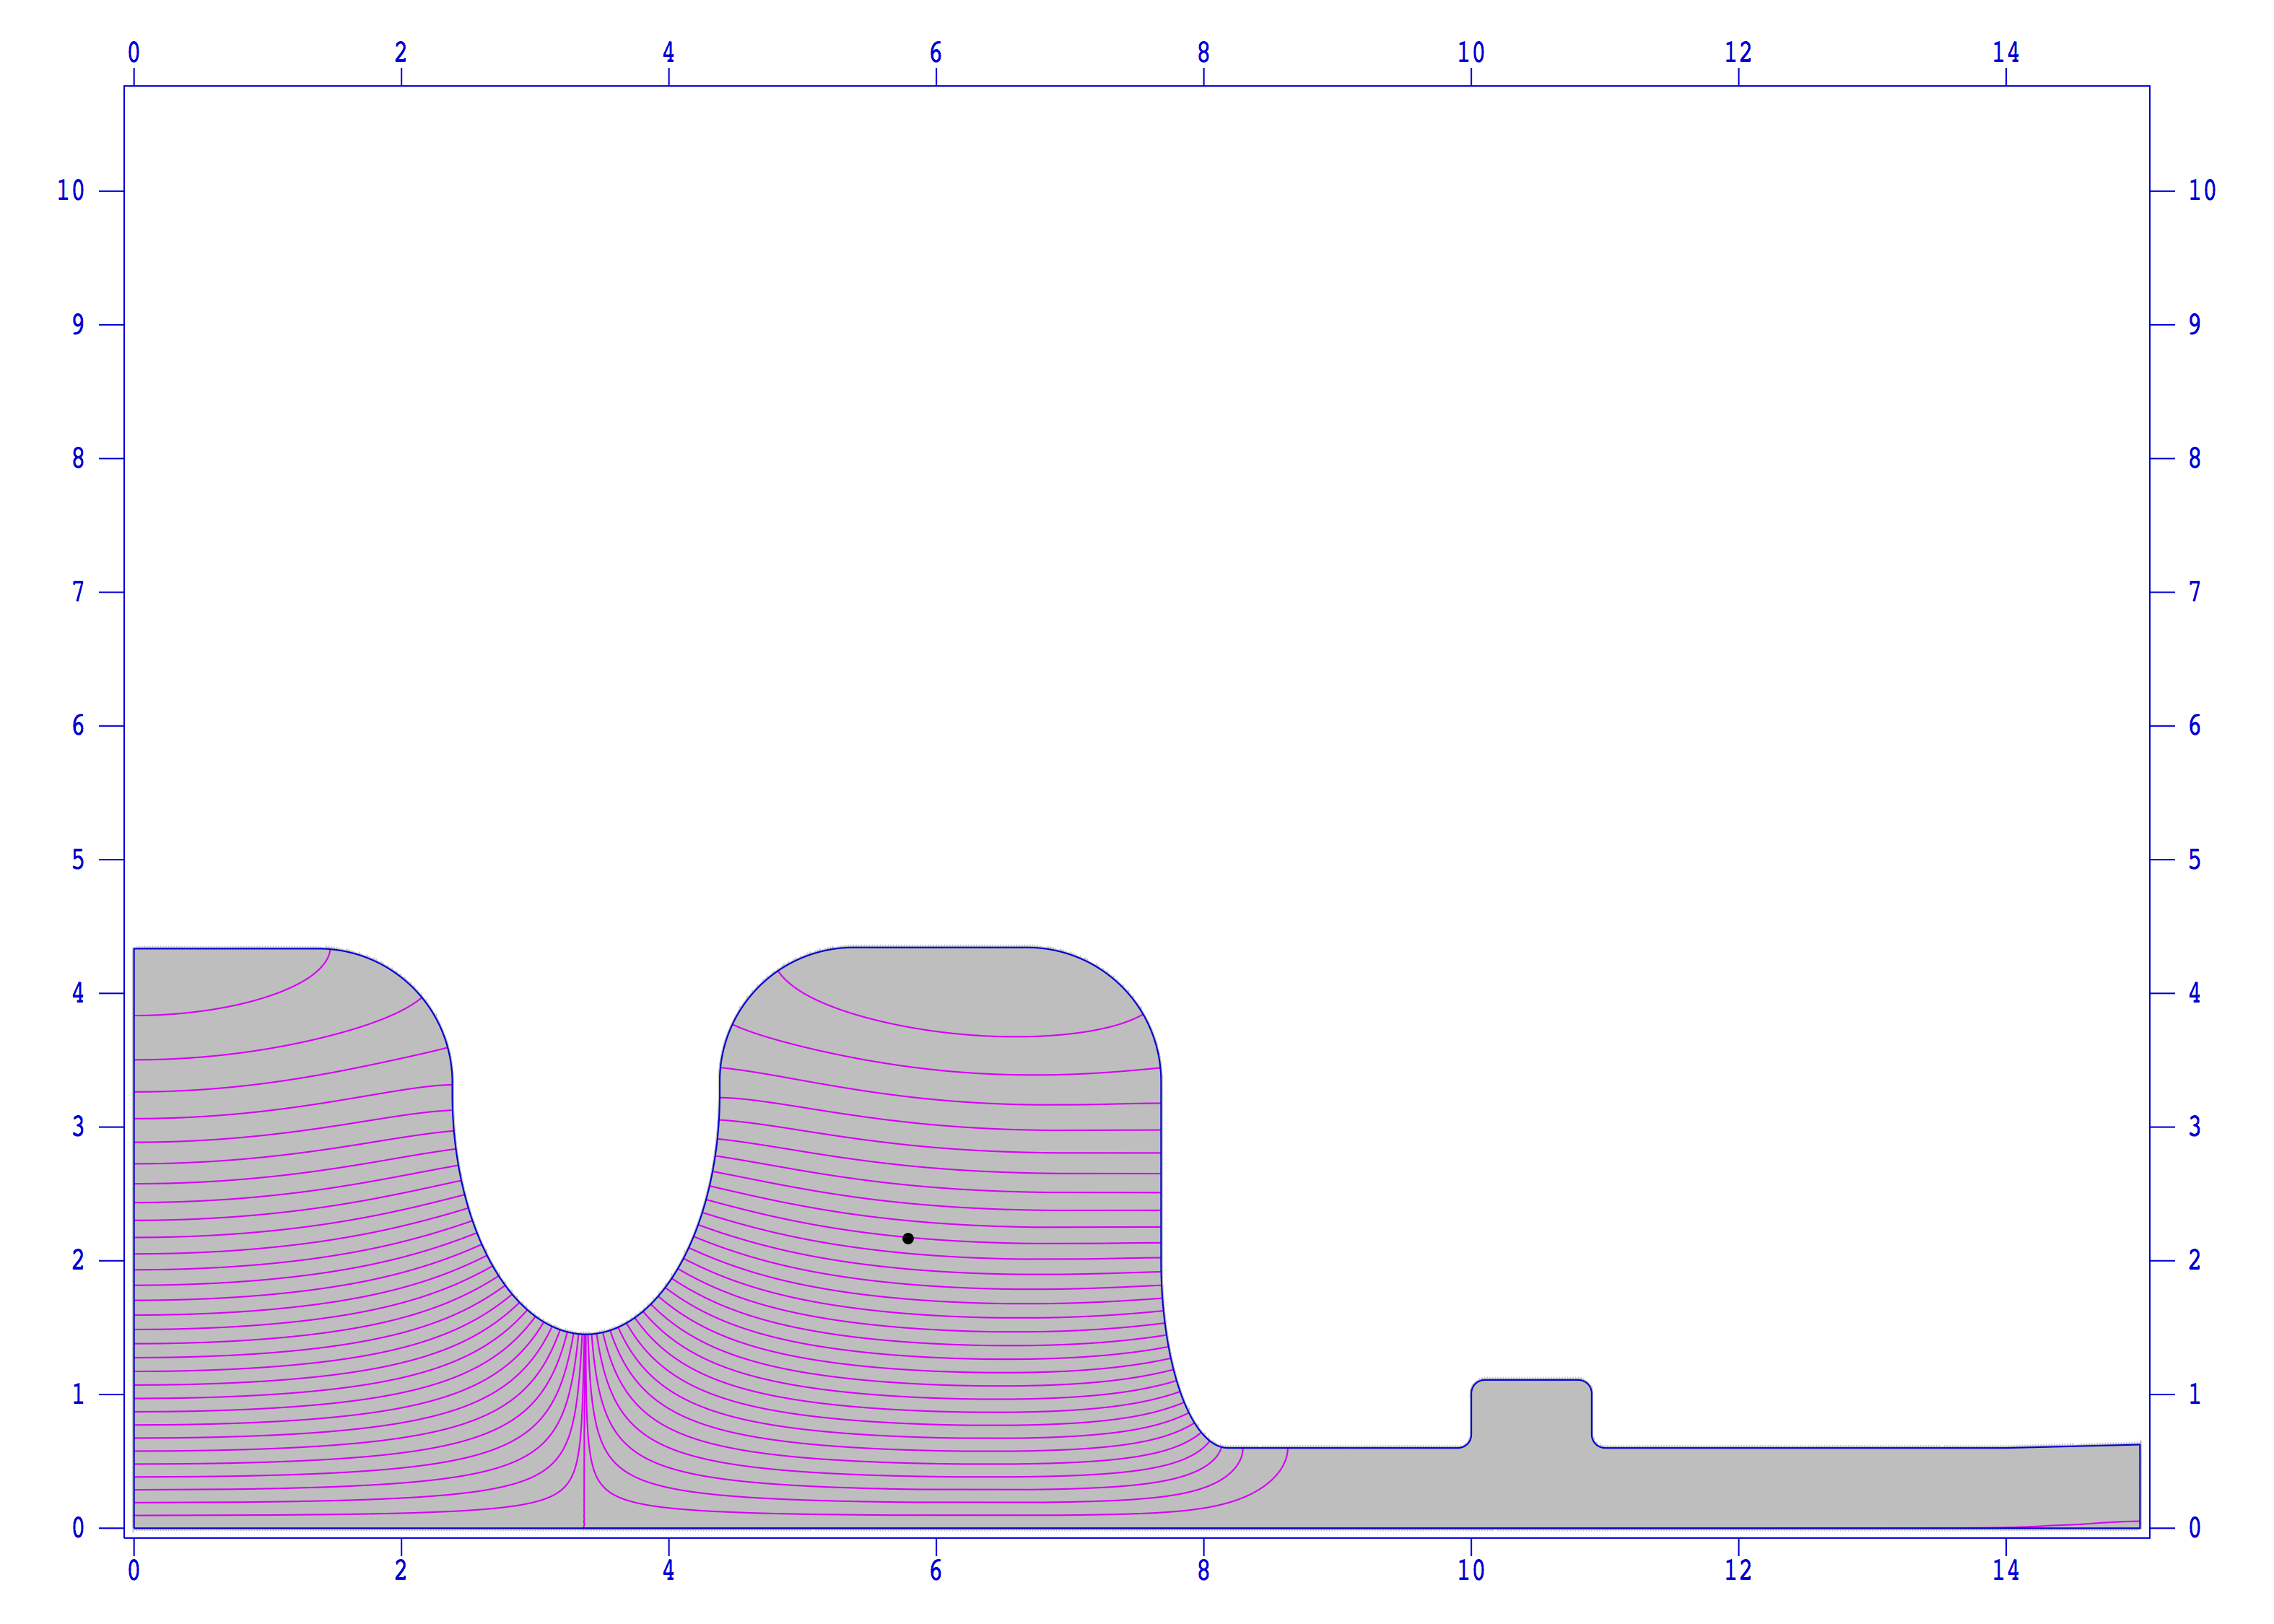
\includegraphics[width=0.45\textwidth]{field_s}
	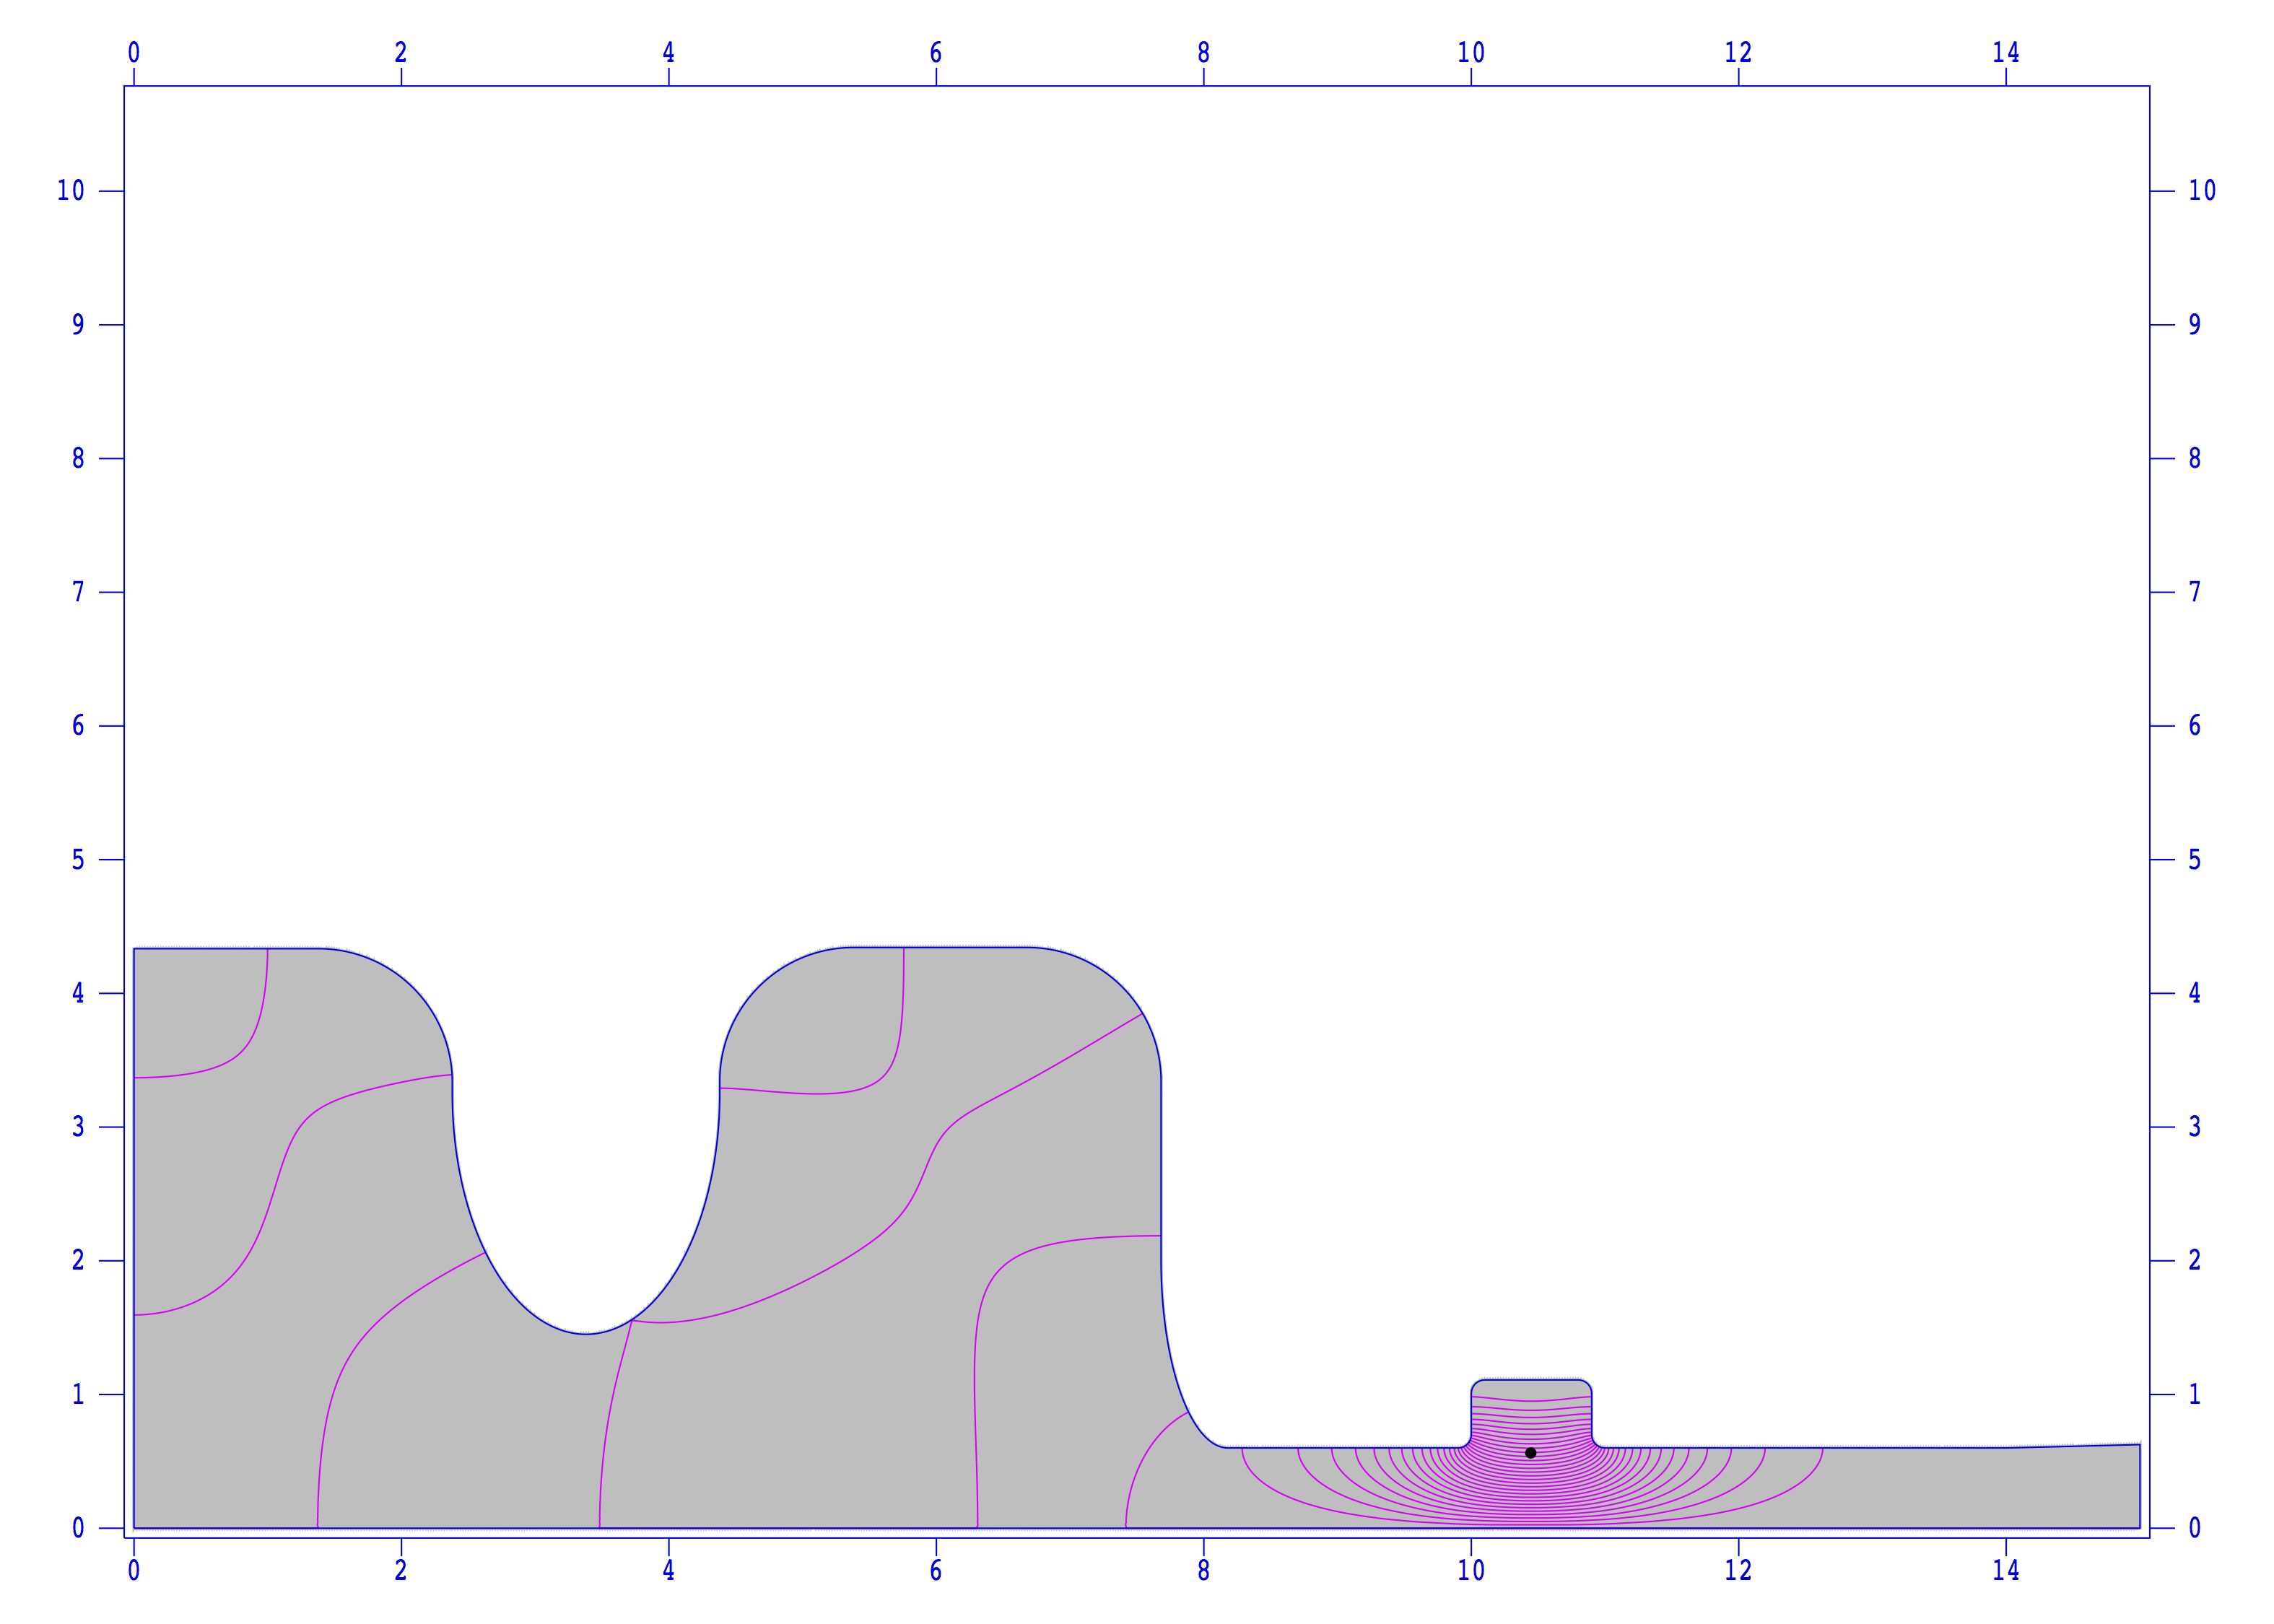
\includegraphics[width=0.45\textwidth]{field_x}
	\caption{
	双频电子枪中的轴线电场分布。左图:S 波段基模电场分布;右图:X 波段高阶模电场分布。}
	\label{fig:field_sx}
\end{figure}

\begin{table}[htbp]
\centering
\caption{\label{tab:geo_s}
S 波段腔结构参数。}
\begin{tabular}{lll}
\toprule
参数 & 值 & 描述\\
\midrule
freq & \SI{2856.00}{MHz} & 微波频率  \\
flatness & 0.9996 & 场平  \\
\midrule
$l_h$ & \SI{3.38}{cm} & 半腔长度  \\
$r_h$ & \SI{4.3341}{cm} & 半腔半径  \\
$c_h$ & \SI{1}{cm} & 半腔倒角半径  \\
$j_h$ & \SI{1}{cm}, \SI{1.8}{cm} & 半腔盘片长、短轴 a、b \\
$l_f$ & \SI{4.8}{cm} & 整腔长度  \\
$r_f$ & \SI{4.3431}{cm} & 整腔半径  \\
$c_f$ & \SI{1}{cm} & 整腔倒角半径  \\
$j_{f, l}$ & \SI{1}{cm}, \SI{1.8}{cm} & 整腔左盘片长、短轴 a、b \\
$j_{f, r}$ & \SI{0.5}{cm}, \SI{1.4}{cm} & 整腔右盘片长、短轴 a、b \\
$r_{f, t}$ & \SI{1.45}{cm} & 束流管道半径  \\
\bottomrule
\end{tabular}
\end{table}

\begin{table}[htbp]
\centering
\caption{\label{tab:geo_x}
X 波段腔结构参数。}
\begin{tabular}{lll}
\toprule
参数 & 值 & 描述\\
\midrule
freq & \SI{11424.25}{MHz} & 微波频率  \\
penetration & $3.02\times10^{-4}$ & 场渗透率  \\
\midrule
$p$ & \SI{9.9}{cm} & 腔起始位置  \\
$l$ & \SI{1.1}{cm} & 腔长度  \\
$r$ & \SI{1.1088}{cm} & 腔半径  \\
$c$ & \SI{0.1}{cm} & 腔倒角半径  \\
$j$ & \SI{0.1}{cm} & 腔盘片半径  \\
$r_t$ & \SI{0.6}{cm} & 束流管道半径  \\
\bottomrule
\end{tabular}
\end{table}

\section{空间分离双频电子枪的动力学验证}
腔型设计好后,需要对双频电子枪的性能进行验证,我们利用 Astra 来做空间分离双频电子枪的动力学模拟。人们真正关心的是注入器出口处束流的参数而非仅仅电子枪出口处的束流参数,因此双频电子枪被放入一个类 LCLS 的光阴极注入器(见图 \ref{fig:injector-x})中进行动力学优化。为验证双频电子枪的亮度提升的效果,需要与普通电子枪的注入器优化结果进行比对。

我们关心的物理量为注入器出口处束流的峰值流强和发射度(100\% 投影发射度,95\% 投影发射度及切片发射度),在束团电荷量一定的情况下(200\,pC),注入器出口处峰值流强可以近似认为只由束团长度决定,因此最终的目标变量设置为注入器出口处束流的 rms 长度与投影发射度。如图 \ref{fig:injector-x} 中所示,整个注入器由双频电子枪,螺线管线圈及两段加速管构成,可优化的变量为:
\begin{itemize}
\item {\sf 激光}:激光长度及横向尺寸
\item {\sf 双频电子枪}:S 波段腔的场强和相位;X 波段腔的场强和相位
\item {\sf 螺线管线圈}:位置和强度
\item {\sf 加速管}:第一段加速管位置和场强;第二段加速管位置和场强
\end{itemize}
其中 S 波段腔的场强应该取可取的最大值,因为阴极表面场越强对空间电荷发射度增长的抑制效果就越好;第二段加速管一般紧贴第一段加速管,因此只要第一段加速管位置确定,第二段的位置也随之确定,不需要优化。从上面的分析看,完整的注入器需要优化 10 个变量,若采用人工方式优化不仅工作量/耗时巨大而且无法保证取到全局最优解。鉴于此,我们采用了遗传算法(Genetic Algorithm,GA)对该多变量问题进行优化。
\begin{figure}[htbp]
	\centering
	
\includegraphics[width=0.9\textwidth]{injector-x}	
	\caption{S/X 双频电子枪的注入器布局示意图。}
	\label{fig:injector-x}
\end{figure}

\subsection{遗传算法优化器}
\subsubsection{NSGA-II}
我们采用了经典而高效的算法 NSGA-II(Nondominated Sorting Genetic Algorithm II)来驱动遗传算法优化器。
\begin{figure}[htbp]
	\centering
	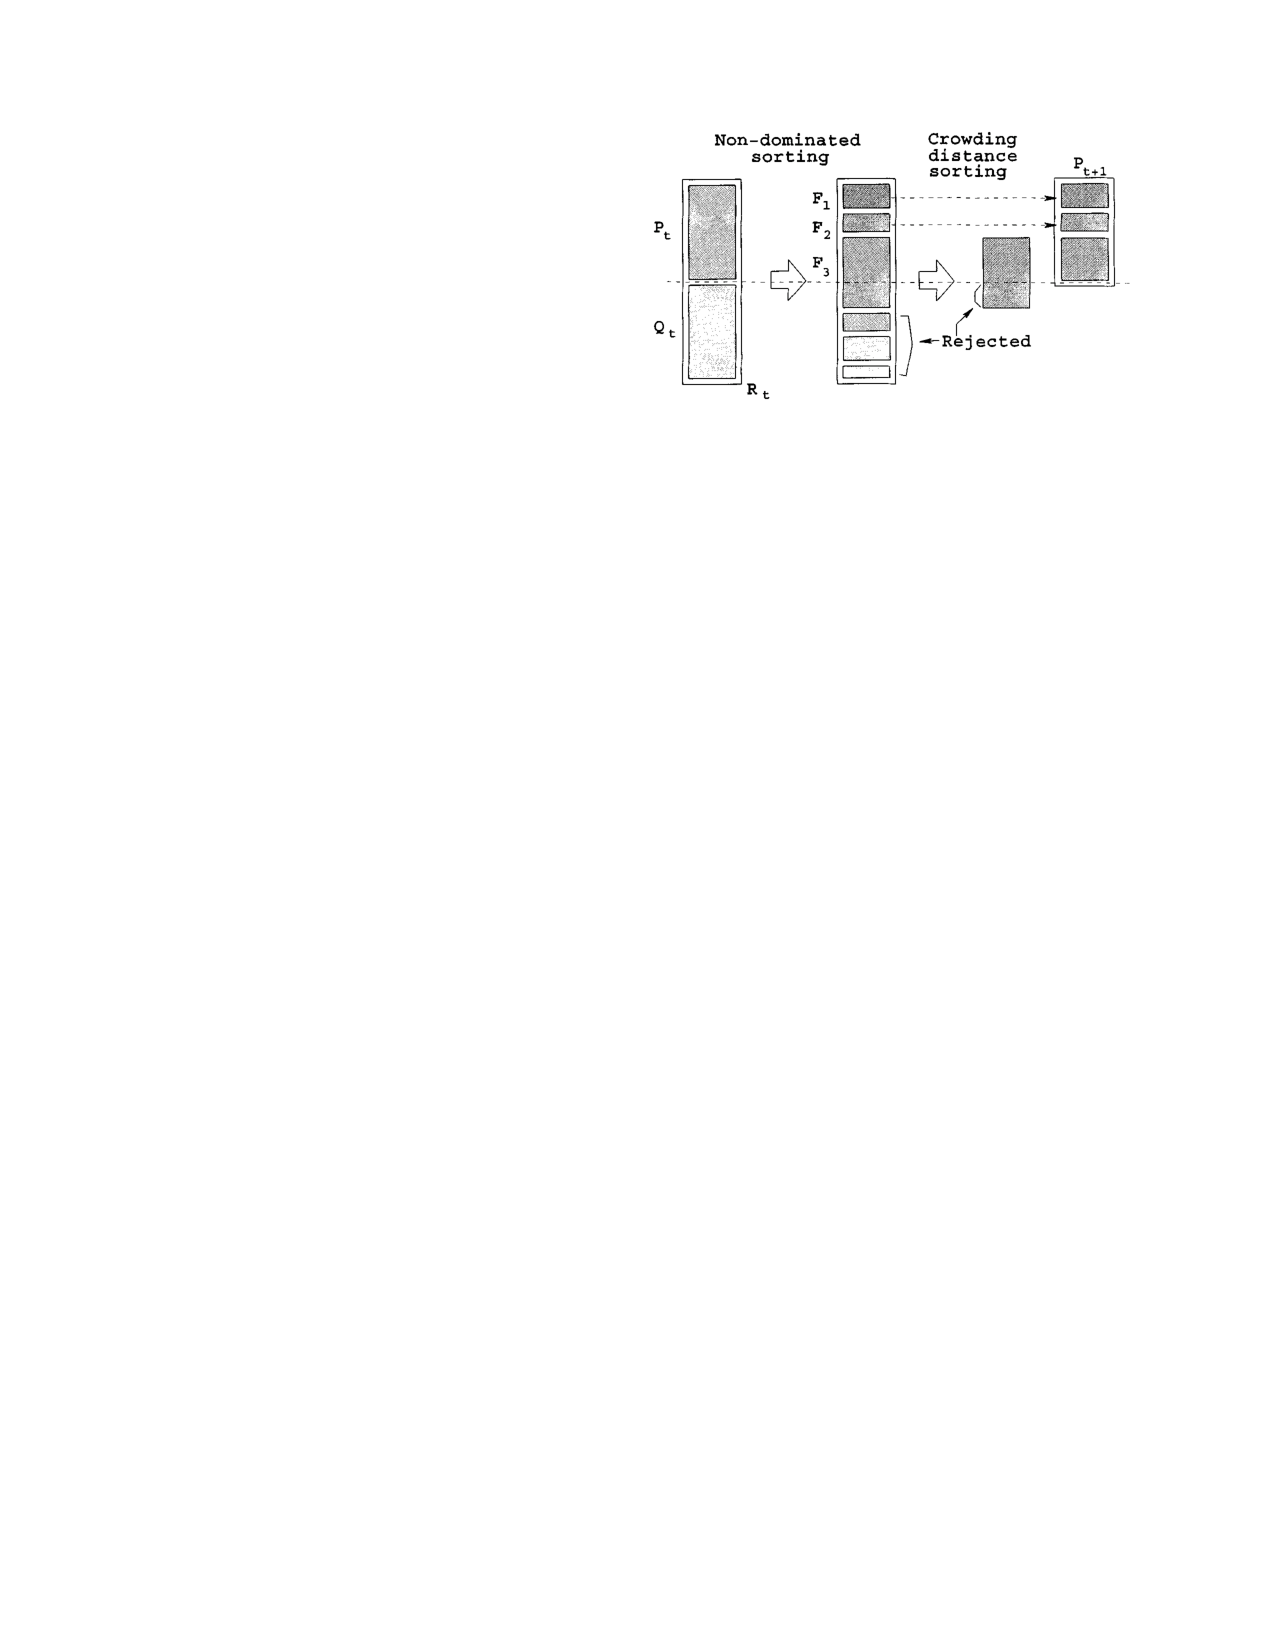
\includegraphics[width=0.6\textwidth]{nsgaii}	
	\caption{NSGA-II 算法原理示意图。}
	\label{fig:nsgaii}
\end{figure}
NSGA-II 的基本原理如图 \ref{fig:nsgaii} 所示,NSGA-II 在进化过程中,同时保留父代和子代,将相邻两代按照种群距离进行筛选,并分为一等公民,二等公民等;产生新的子代时,先从一等公民中按性状优良程度挑选,再依法炮制挑选二等公民,直至达到种群数量上限;新挑选出的子代再分成两组进行 crossover。上述过程一直进行下去,直至种群收敛,此时算法将给出一组最优解,即 Pareto 前沿。多次改变初始种群进行 NSGA-II,就可以获得全局最优解集。

\subsubsection{遗传算法优化器逻辑结构}
遗传算法优化器逻辑上分为四部分:生成器,运行器,后处理器以及迭代器。下面首先介绍优化器的运行方式,再分别介绍四部分各自的用途。

优化器需要一个已经运行通过的模拟算例作为起始算例,该模拟算例一般体现为一个文件夹,其中包含模拟的输入文件,以及模拟所需要的场分布等附加文件。优化器运行时,对初始算例中的输入文件进行解析,给出输入文件中所有重要的可变参数,随后根据优化器配置文件中设置的具体关心的参数以及各参数的可变范围,依据初始算例,对其参数进行覆盖,随机生成给定数量的初始种群。随后优化器调用动力学模拟程序(例如 Astra)对初始种群的每个个体进行模拟,模拟结束后对模拟结果进行后处理,最后该种群的后处理结果经过汇总分析后,产生新一代种群,依此类推,直到达到优化目标或超出预设资源(时间/存储空间等),优化结束。

\red{这里要插一张流程图。}

在上面的过程中,生成器会根据迭代器提供的输入参数,基于初始算例给出新的待模拟算例;运行器负责调用动力学模拟软件对生成器给出的待模拟算例进行模拟;后处理器接受运行器模拟完成的算例,并对模拟结果进行统计,得到关心的参数(例如注入器出口处束长,发射度等);迭代器则扮演了优化过程的大脑的角色,它根据后处理器给出各算例的参数,给出下一组待模拟算例的输入参数(例如激光尺寸,腔的相位、强度等),同时迭代器还承担着控制整个优化进程的任务,也即它需要根据情况判断是否优化条件达成,是否超时/超储存空间而中止优化等。

以上是遗传算法优化器的一般逻辑结构,该结构并不仅限于遗传算法优化,而是适用于几乎一切加速器中的束流动力学模拟优化任务。在处理不同任务时,只需要根据优化目标和优化方法对迭代器进行定制即可。例如,要对束线中某个参数进行扫描,那么迭代器的逻辑就是根据待扫描参数的上一个取值,给出待扫描参数的下一个取值;对于支持并行计算的平台,实现可以更加简单和快速:迭代器初始化时直接给出待扫描参数全部可能取值,那么该扫描任务一次迭代就完成了。对于本章所采用的遗传算法而言,迭代器执行遗传算法的筛选过程,将父代中符合要求的个体留下,crossover/变异后产生下一代种群。

上面描述的优化器逻辑结构也自动具有扩展功能:例如运行器可以支持调用各种模拟软件,如 Astra,GPT,Parmela 等,只需要为相应的模拟软件写好调用接口即可;而迭代器的具体实现也可以多种多样,甚至可以由人来担任迭代器,根据后处理器给出的上一代性能,决定下一代的优化方向。

\subsubsection{遗传算法优化器的编程实现}
我们采用 Python 编程实现了遗传算法优化器的逻辑结构。

\subsection{遗传算法优化平台}
为保证优化时间在可接受的范围内,我们采用了清华大学探索 100 高性能计算平台作为遗传算法优化器的运行平台。探索 100 百万亿次集群计算机,共有 740 个计算节点,8800 个处理器核,处理器采用 Intel Xeon 5670,系统的理论浮点峰值计算性能达到 104\,TFlops,存储总容量达 1000\,TB。另外,该系统还配置了 17 个 Nvidia Tesla S1070 的 GPU 系统,计算能力达 68\,TFlops。探索 100 是国内最先进的超级计算机之一,其计算能力 2011 年在全国高校居首位。

\red{平台的基本设置和参数}

\subsection{基于遗传算法的双频电子枪注入器动力学优化}

\begin{figure}[htbp]
	\centering
	
\includegraphics[width=0.9\textwidth]{injector-c}	
	\caption{分离型 S/C 双频电子枪的注入器布局示意图。}
	\label{fig:injector-c}
\end{figure}

\subsubsection{S/C-band rf gun}
In this section, a two frequency gun of split configuration, in which the solenoid is located in between the S-band RF gun and the C-band buncher, is investigated by the genetic optimizer for the \SI{200}{pC} case.

The photoinjector layout shown in Fig.~\ref{fig:injector-c} is modified based on the conventional S-band photoinjector, including a BNL type S-band RF gun (\SI{120}{MV/m}), an emittance compensation solenoid, a C-band buncher and two S-band travelling wave linacs ($<$ \SI{78}{MV} per linac). The photocathode laser distribution is longitudinally flattop with rising and falling time equal to 10\% of the pulse length, transversely Gaussian with radius truncated at one sigma. The laser dimensions, gun phase, solenoid strength, C-band buncher location, gradient, phase, booster linac gradient and position are optimization parameters for the optimizer. As shown in Fig.~\ref{Pareto120}, the 100\% emittance and RMS bunch length at injector exit are minimized with beam energy constrained above \SI{100}{MeV} at injector exit. The \SI{0.65}{mm} RMS bunch length corresponds to \SI{30}{A} peak current for \SI{200}{pC}. Fig.~\ref{Pareto120} shows, with a C-band buncher added, emittance at injector exit can be reduced by $\sim$25\% at \SI{30}{A} peak current. Besides, Fig.~\ref{Pareto120} (b) also shows the cathode emittance are almost the same as the 95\% emittance, which means the transverse beam brightness at cathode is preserved to the injector exit.

\begin{figure}[htbp]
	\centering
	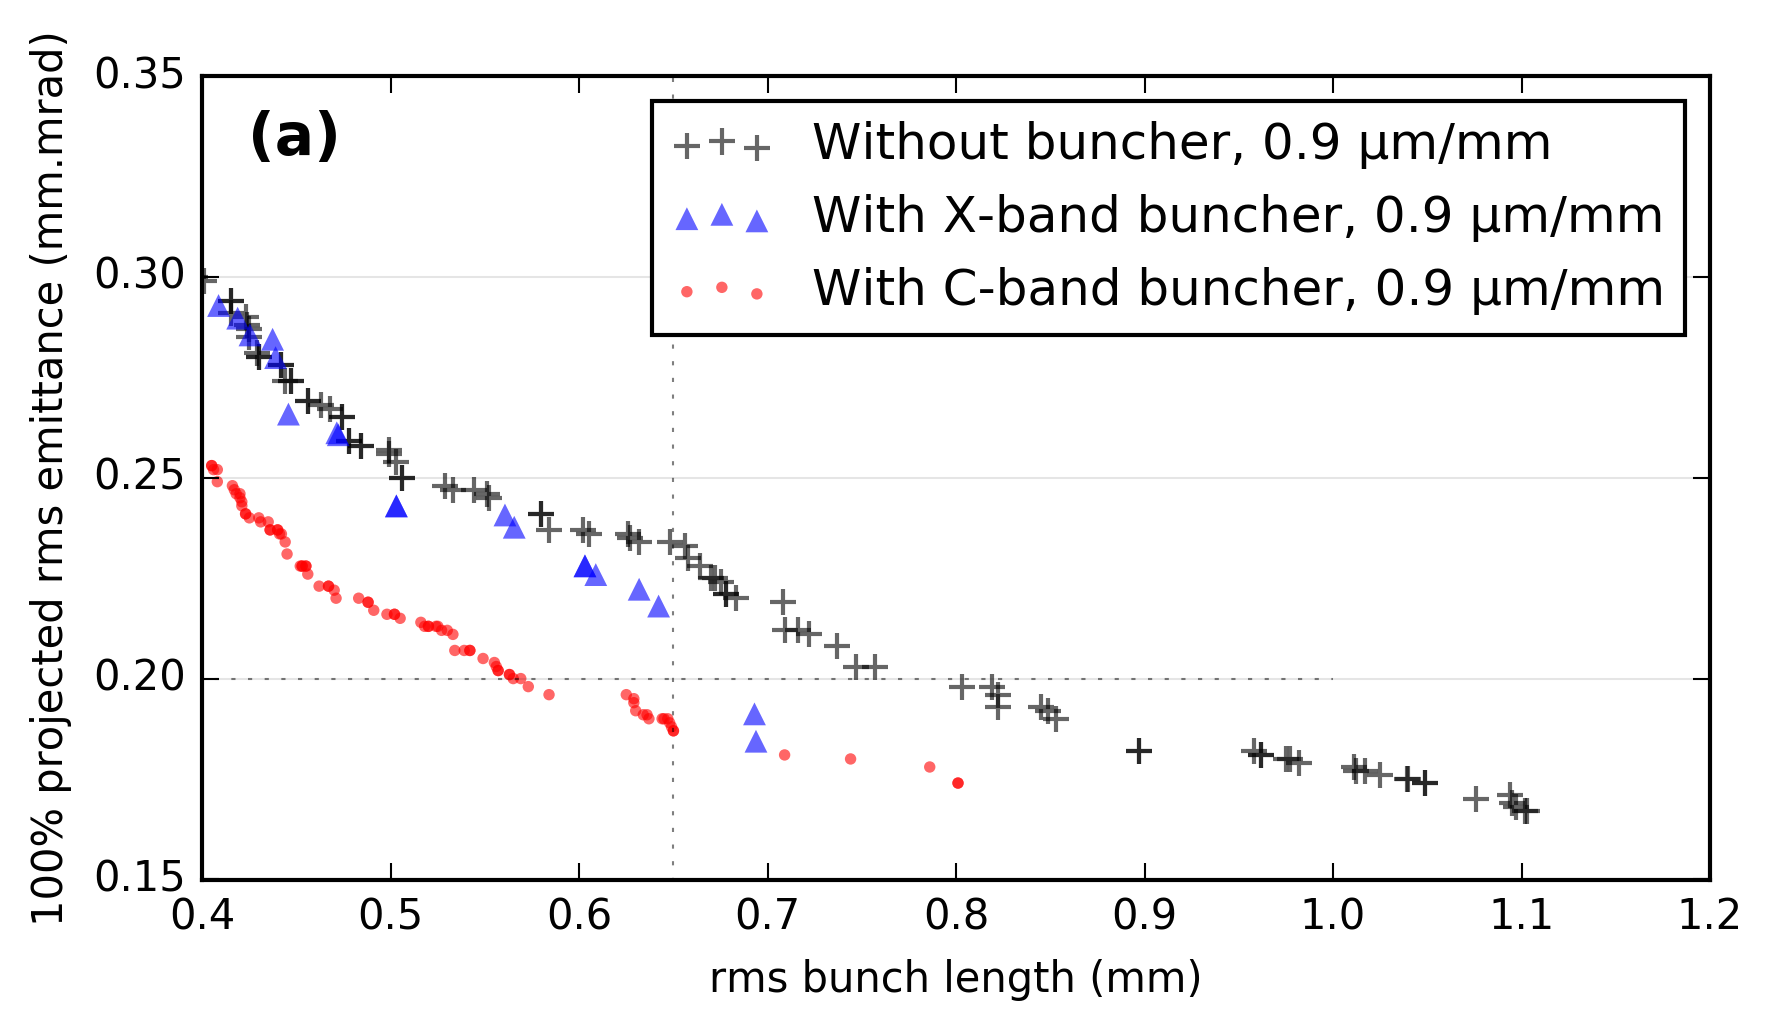
\includegraphics[width=0.6\textwidth]{s120-a}\\
	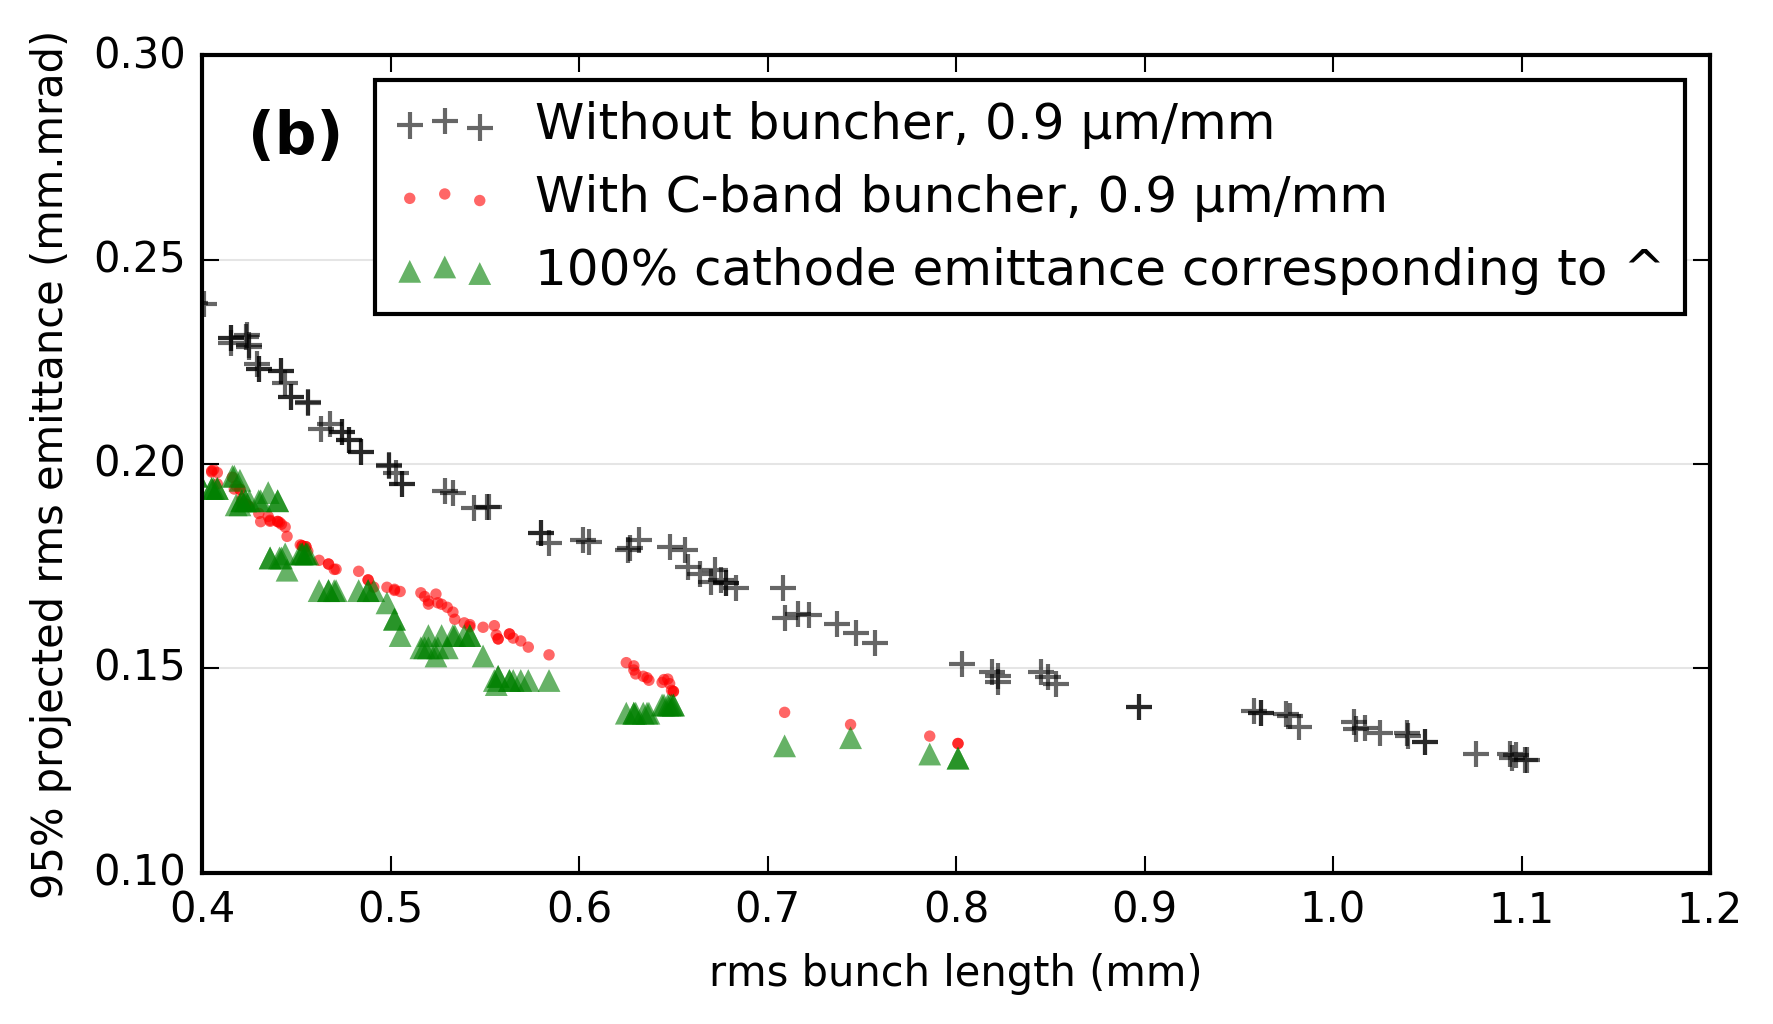
\includegraphics[width=0.6\textwidth]{s120-b}
	\caption{
	200\,pC 束团发射度 vs. rms 长度的一组最优解集。Astra 模拟中采用 10000 宏粒子。图中同时比较了 S 波段光阴极注入器加入 C 波段高频腔与否的发射度优化情形。}
	\label{Pareto120}
\end{figure}

Fig.~\ref{laser_dimension} shows why the transverse emittance is reduced after a C-band buncher is added into the S-band photoinjector. With a buncher compressing bunch length downstream of the gun, the beam peak current at cathode can be lower, so laser duration can be longer and laser radius can be smaller, and emittance contributed by the cathode are then reduced. Corresponding to \SI{30}{A} peak current, the laser pulse duration increased from \SI{5}{ps} to \SI{10}{ps}, and laser radius reduced from \SI{0.4}{mm} to \SI{0.32}{mm}. According to the charge saturation in the ``cigar'' regime, the laser duration is inversely proportional to $R^{3/2}$, so a laser radius reduction of 37\% is expected, instead, a 20\% reduction is chosen by optimizer, which means the laser dimensions chosen by optimizer are a bit off the max cathode transverse brightness after a buncher is added, unlike the case without a buncher. Besides, the max laser pulse lengths chosen by the optimizer for both with and without buncher cases are below  15 ps, which is suspicious and may be caused by chromatic effects or other reasons, such issues will be investigated in future in order to further reduce beam emittance.

The slice emittance of the \SI{30}{A} solutions in Fig.~\ref{Pareto120} are shown in Fig.~\ref{slice_emittance}, which shows a core slice emittance of \SI{0.15}{\mu m} after a buncher is added, a 25\% reduction compared to the no buncher case. After the thermal emittance is reduced from 0.9 to \SI{0.5}{\mu m/mm}, the core slice emittance is further reduced to \SI{0.1}{\mu m}.

\begin{figure}[htbp]
	\centering
	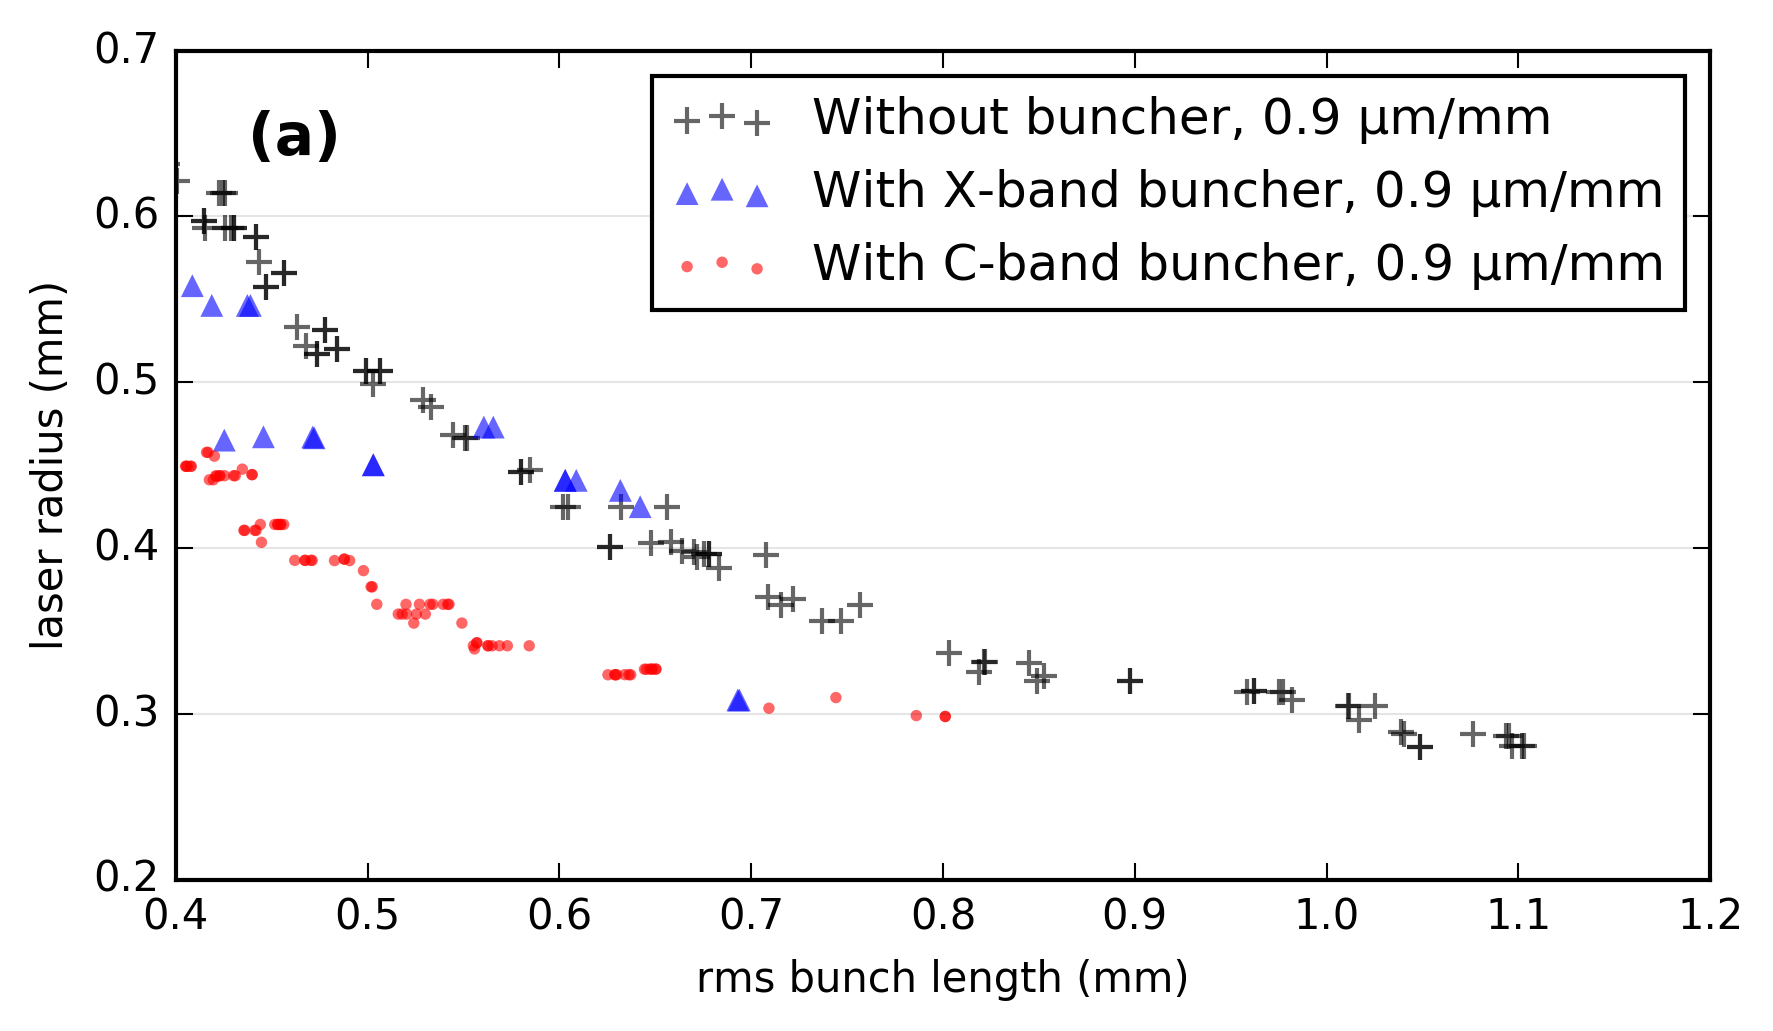
\includegraphics[width=0.6\textwidth]{laser-a}\\
	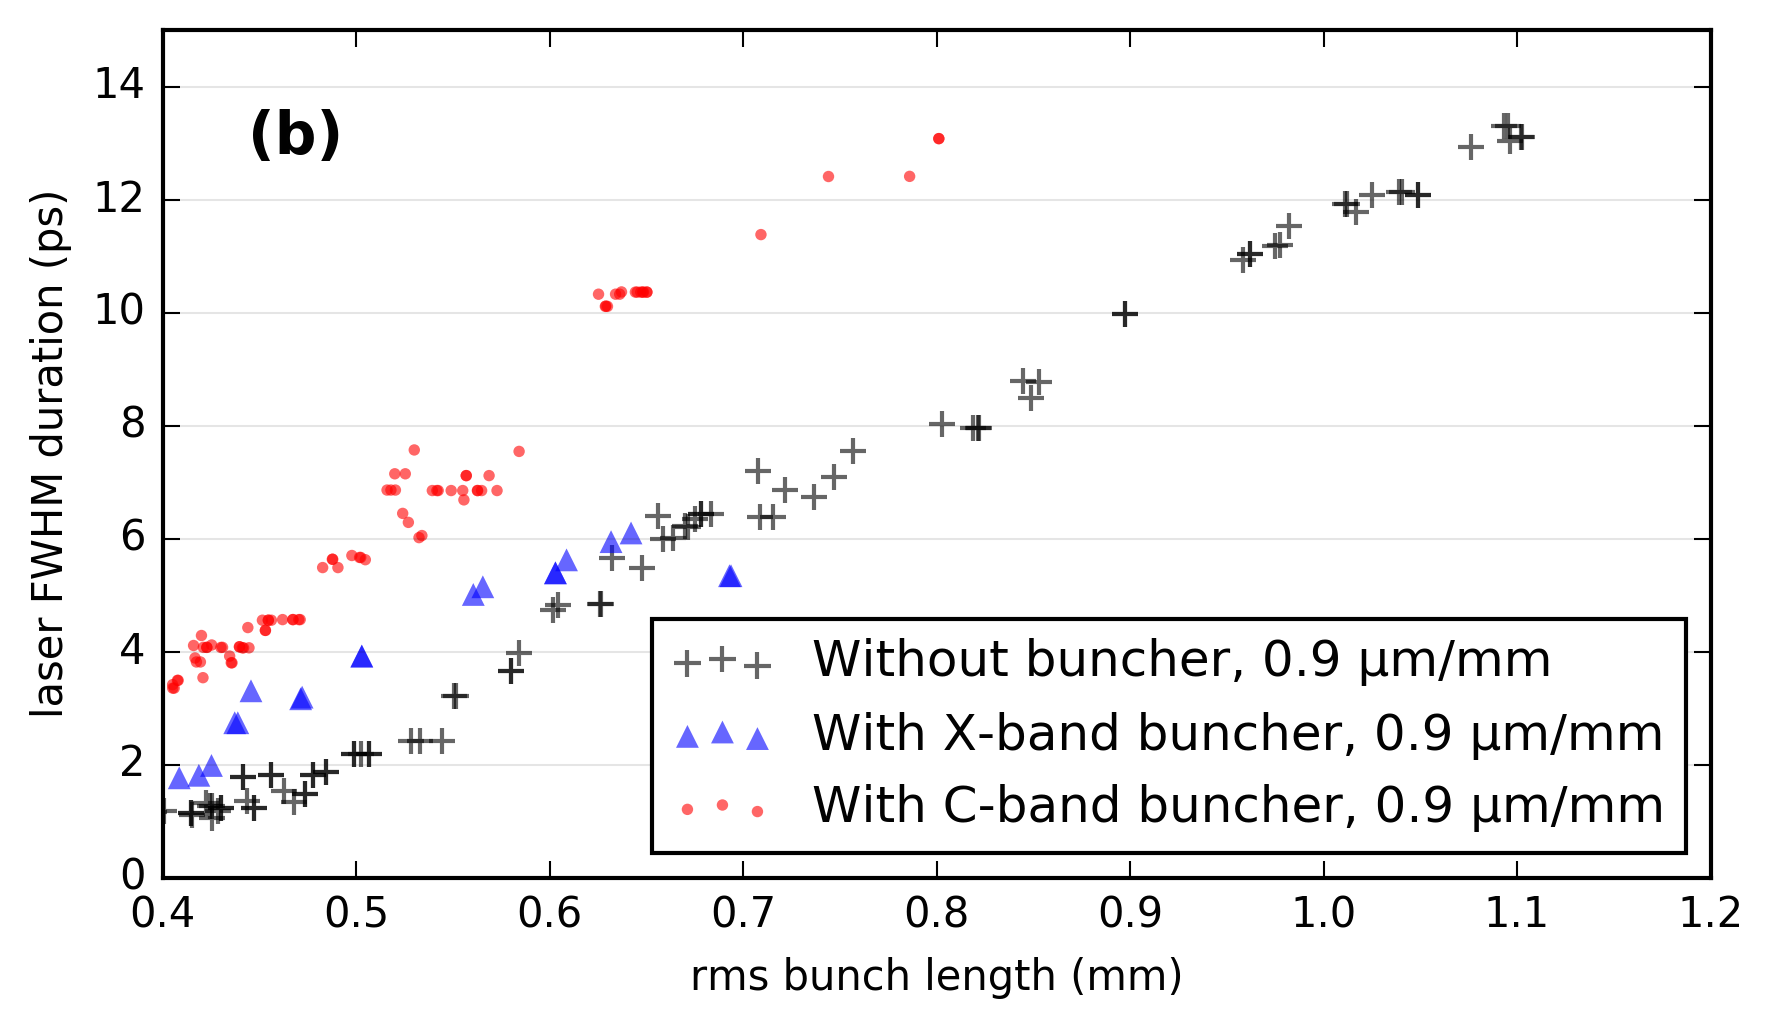
\includegraphics[width=0.6\textwidth]{laser-b}
	\caption{图 \ref{Pareto120} 给出优化结果所对应的激光半径和 FWHM 长度。}
	\label{laser_dimension}
\end{figure}

\begin{figure}[htbp]
	\centering
	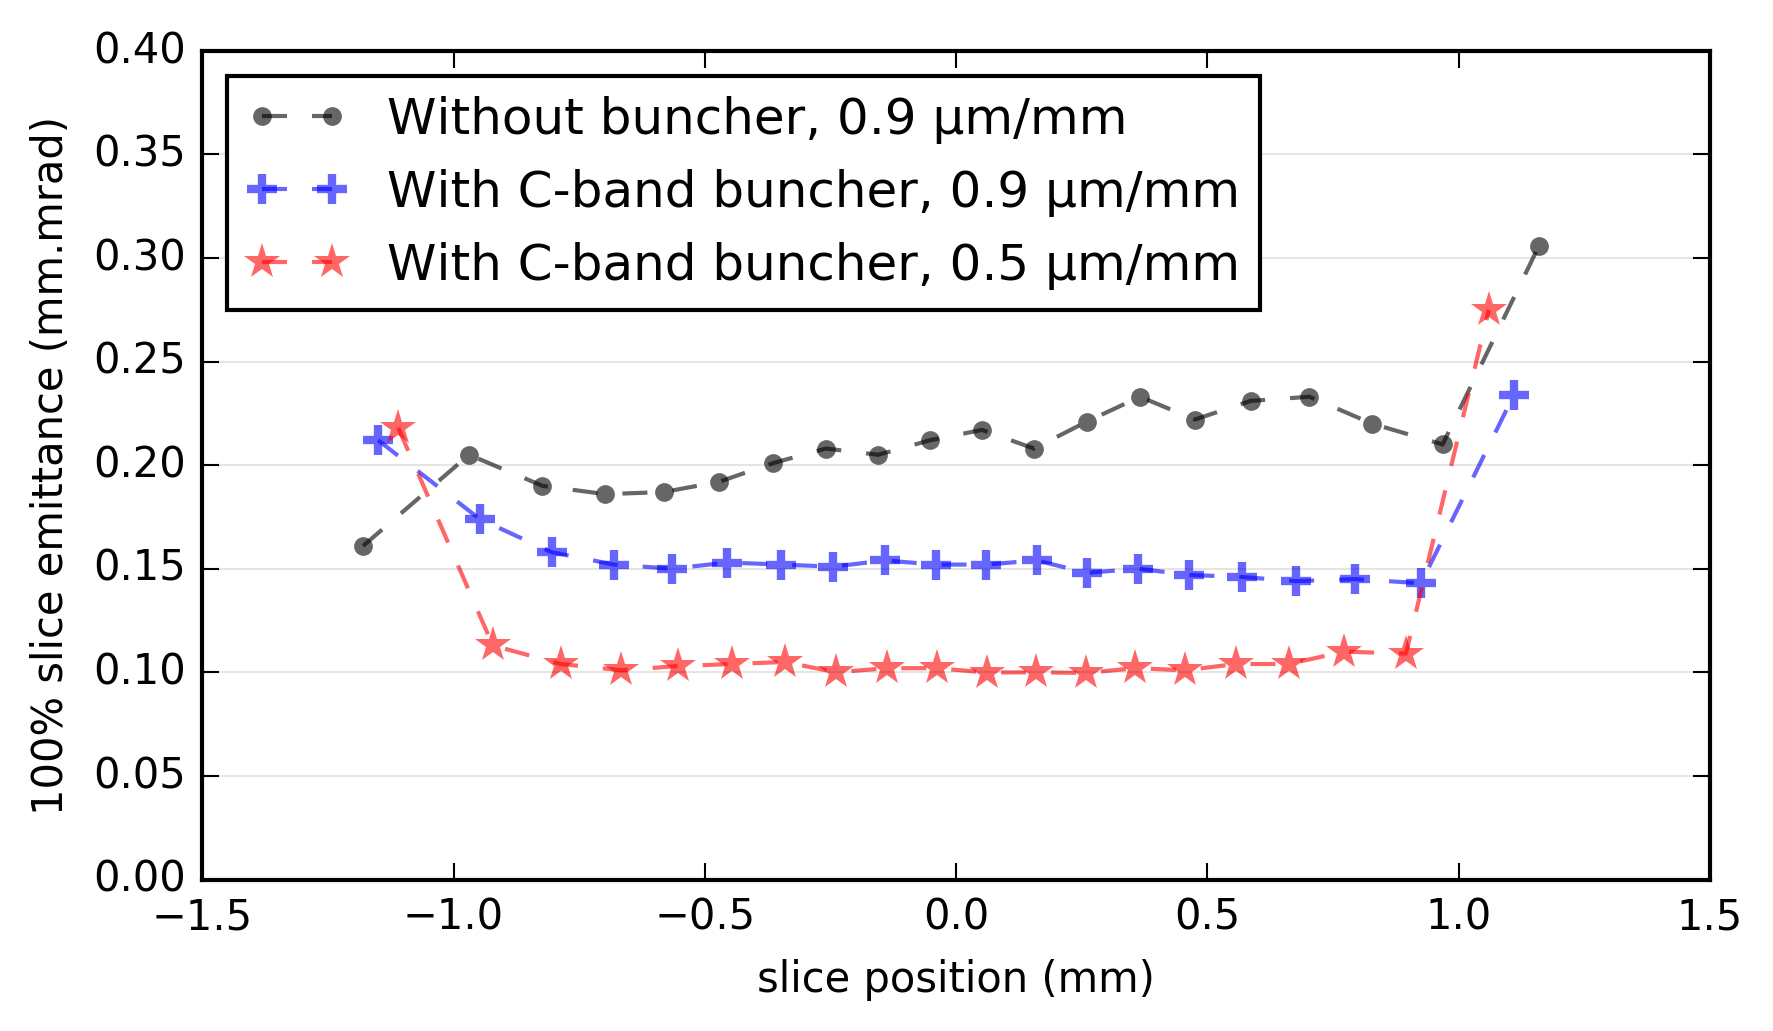
\includegraphics[width=0.6\textwidth]{slice}
	\caption{\SI{200}{pC} 束团,注入器出口处 \SI{30}{A} 峰值流强的优化解的切片发射度。Astra 模拟中采用了 20000 宏粒子。}
	\label{slice_emittance}
\end{figure}

\subsubsection{S/X-band rf gun}
In this section, a two frequency RF gun of combined configuration is investigated by the GA optimizer for the \SI{200}{pC} case. The injector layout is shown in Fig.~\ref{fig:injector-x}. The multivariate optimization settings are almost identical to the previous presented S/C-band gun case, except for the longitudinal distribution which is uniform in the S/X-band gun case.

Fig.~\ref{Pareto120} (a) shows the optimized Pareto front of the S/X-band gun injector compared with the S/C-band gun injector one. The Pareto front with the X-band buncher is better than the one without buncher and approach to the one with C-band split buncher when rms bunch length > \SI{0.65}{mm} (corresponding to peak current < \SI{30}{A}). The reason why the split gun dominates the combined gun in regard of emittance reduction with peak current $\ge$ \SI{30}{A} remains to be investigated.

\subsubsection{高频腔选取不同波段的优化结果对比}

\subsubsection{分离型和合并型双频电子枪性能差异的分析}

\section{非线性发射区注入器束流亮度的研究}

\section{小结}
By adding a harmonic buncher either before or after the emittance compensation solenoid, a two frequency photoinjector is proposed to further improve beam brightness by using cigar beam photoemission. Both the initial RF design and beam dynamics investigations with a GA optimizer are presented. The preliminary simulation results show that with a HOM cavity added, the emittance at injector exit can be reduced by $\sim$25\% at \SI{30}{A} peak current for \SI{200}{pC}, and slice emittance can be reduced to $\sim$\emit{0.10} with a  \SI{0.5}{\mu m/mm} thermal emittance. Nevertheless there're several issues yet to be solved. To name a few, the GA optimizer chooses not to take full advantage of the buncher by lengthening the laser pulse beyond \SI{10}{ps}; putting the buncher downstream the solenoid could achieve smaller emittance compared with buncher before the solenoid. We would continue to investigate the mechanisms behind all these issues in order to further improve the beam emittance.
